\documentclass[aspectratio=169]{beamer}
\usetheme[faculty=phil]{fibeamer}
\usepackage{polyglossia}
\setmainlanguage{english} %% main locale instead of `english`, you
%% can typeset the presentation in either Czech or Slovak,
%% respectively.
\setotherlanguages{russian} %% The additional keys allow
%%
%%   \begin{otherlanguage}{czech}   ... \end{otherlanguage}
%%   \begin{otherlanguage}{slovak}  ... \end{otherlanguage}
%%
%% These macros specify information about the presentation
\title[AGLA2]{Analytical Geometry and Linear Algebra II, Lab 9} %% that will be typeset on the
\subtitle{Eigenvalues and Eigenvectors \\ Diagonalization of a Matrix \\ Difference equation
         } %% title page.
\author{Oleg Bulichev}
%% These additional packages are used within the document:
\usepackage{ragged2e}  % `\justifying` text
\usepackage{booktabs}  % Tables
\usepackage{tabularx}
\usepackage{tikz}      % Diagrams
\usetikzlibrary{calc, shapes, backgrounds}
\usepackage{amsmath, amssymb}
\usepackage{url}       % `\url`s
\usepackage{listings}  % Code listings
% \usepackage{subfigure}
\usepackage{floatrow}
\usepackage{subcaption}
\usepackage{mathtools}
\usepackage{todonotes}
\usepackage{fontspec}
\usepackage{multicol}
\usepackage{pdfpages}
\usepackage{wrapfig}
\usepackage{animate}
\usepackage{booktabs}
\usepackage{multirow}

\graphicspath{{resources/}}
\frenchspacing

\setbeamertemplate{caption}[numbered]
\usetikzlibrary{graphs}

% \usepackage[backend=biber,style=ieee,autocite=footnote]{biblatex}
% \addbibresource{biblio.bib}
% \DefineBibliographyStrings{english}{%
%   bibliography = {References},}

\newcommand{\oleg}[2][] {\todo[color=red, #1] {OLEG:\\ #2}}
\newcommand{\fbckg}[1]{\usebackgroundtemplate{\includegraphics[width=\paperwidth]{#1}}}%frame background

\usepackage[framemethod=TikZ]{mdframed}
\newcommand{\dbox}[1]{
\begin{mdframed}[roundcorner=3pt, backgroundcolor=yellow, linewidth=0]
\vspace{1mm}
{#1}
\vspace{1mm}
\end{mdframed}
}

\begin{document}
\setlength{\abovedisplayskip}{0pt}
\setlength{\belowdisplayskip}{0pt}
\setlength{\abovedisplayshortskip}{0pt}
\setlength{\belowdisplayshortskip}{0pt}

\fbckg{fibeamer/figs/title_page.png}
\frame[c]{\setcounter{framenumber}{0}
    \usebeamerfont{title}%
    \usebeamercolor[fg]{title}%
    \begin{minipage}[b][6.5\baselineskip][b]{\textwidth}%
        \textcolor{black}{\raggedright\inserttitle}
    \end{minipage}
    % \vskip-1.5\baselineskip

    \usebeamerfont{subtitle}%
    \usebeamercolor[fg]{framesubtitle}%
    \begin{minipage}[b][3\baselineskip][b]{\textwidth}
        \raggedright%
        \insertsubtitle%
    \end{minipage}
    \vskip.25\baselineskip
}
%   \frame[c]{\maketitle}

\fbckg{fibeamer/figs/common.png}

\begin{frame}[c]{How I spent last weekend}
    \framesubtitle{}
    \begin{figure}[H]
        \begin{subfigure}{0.49\textwidth}
            \centering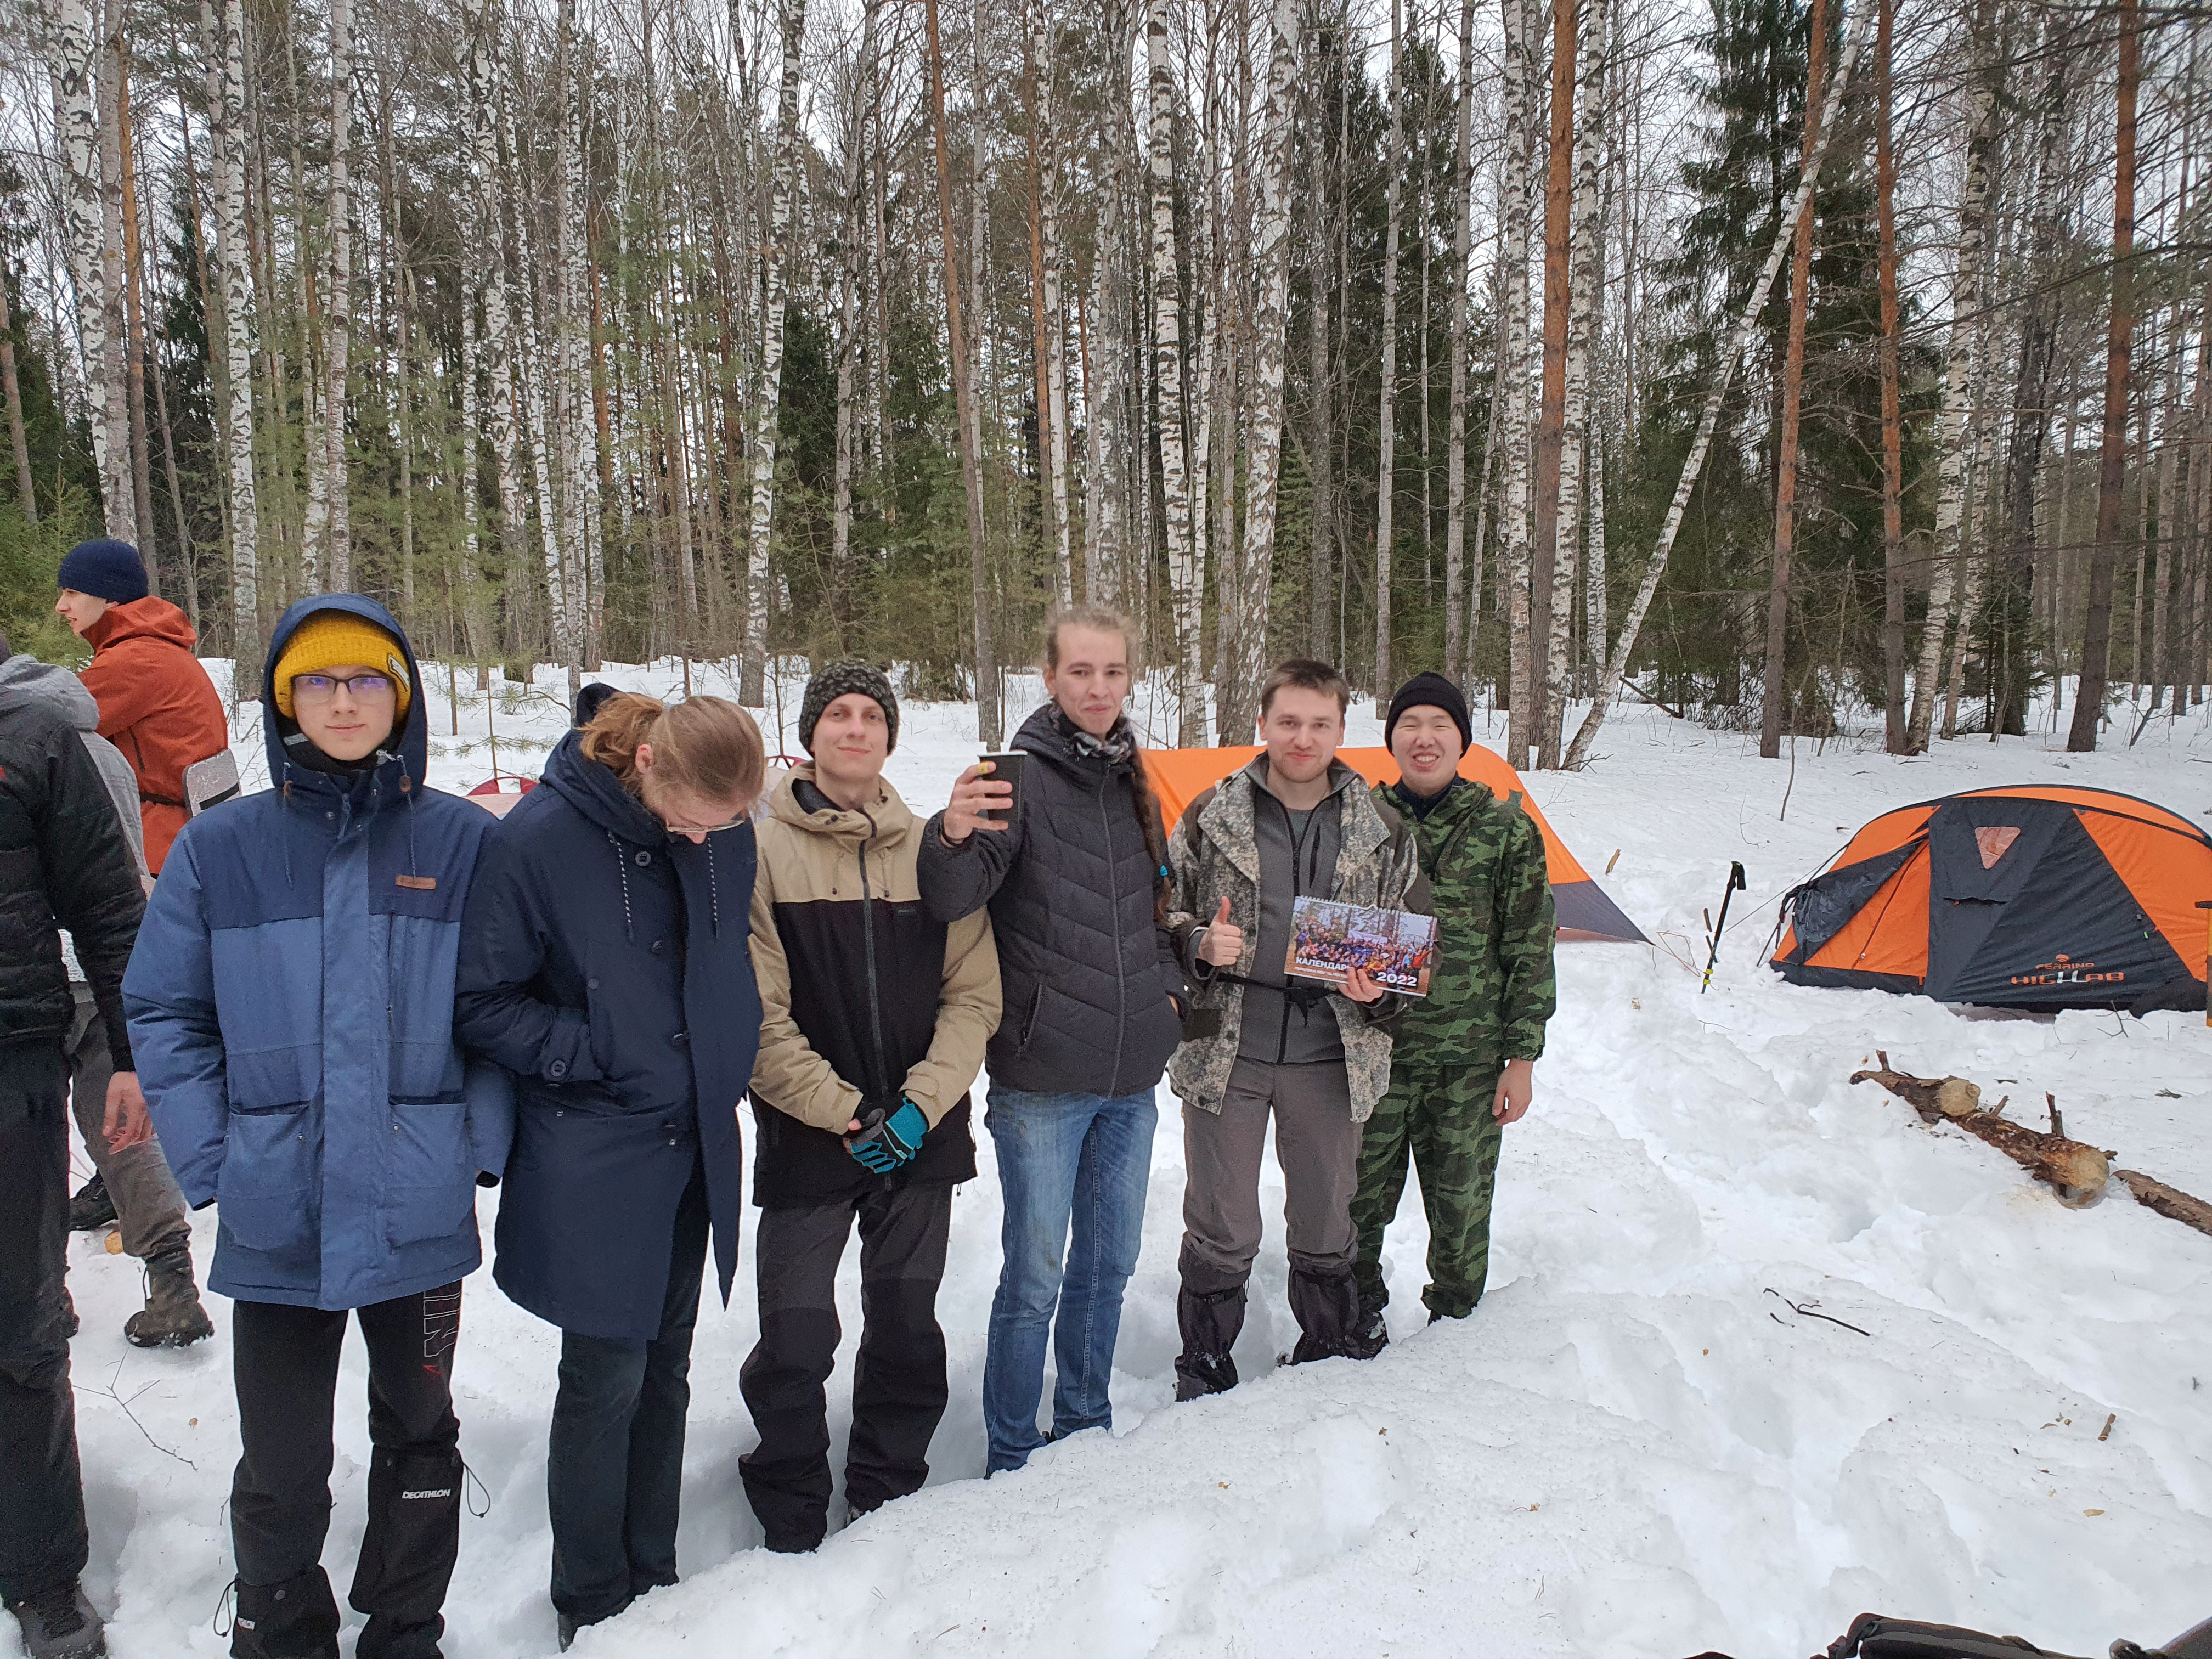
\includegraphics[height=5cm,width=1\textwidth,keepaspectratio]{flex_1.JPG}
        \end{subfigure}
        \hfill
        \begin{subfigure}{0.49\textwidth}
            \centering\includegraphics[height=5cm,width=1\textwidth,keepaspectratio]{flex_2.JPG}
        \end{subfigure}
        \caption*{\Large Hiking Club KFU "Tochka" event }
    \end{figure}
\end{frame}

\begin{frame}[t]{Where it can be used}
\framesubtitle{}
    \begin{itemize}
        \item Machine learning (transform data in more suitable usage)
        \item Make some calculations easier (matrix$^100$ – piece of cake)
        \item Predict the behavior of linear systems (physics, biology, etc)
        \item Design the controller for our system
        \item Estimate the complexity of calculations
        \item ...
    \end{itemize}
\end{frame}

\begin{frame}[t]{Definition}
\framesubtitle{}
\Large 
In linear algebra, an \textbf{eigenvector or characteristic vector }of a linear transformation is a non-zero \textit{vector that changes by only a scalar factor when that linear transformation is applied to it}. \beamerbutton{\href{https://en.wikipedia.org/wiki/Eigenvalues_and_eigenvectors}{Wiki}}
\bigskip

$ A\mathbf{x}=\lambda\mathbf{x}$, where \\ 
$x$ -- eigenvector (should be non-zero), \\ 
$\lambda$ -- eigenvalue, \\ 
$A$ -- \textit{square} matrix. \\ 
For $n \times n$ matrix -- max amount of $\lambda$ is a number of $n$ .
\end{frame}

\begin{frame}[t]{EigenValues concept}
    \framesubtitle{Video}
    \vspace{-0.6cm}
    \begin{figure}[H]
        \href{https://youtu.be/PFDu9oVAE-g}{
            \centering\includegraphics[height=6cm,width=1\textwidth,keepaspectratio]{eigenvideo_brown.jpg}}
        % \caption{Click on a picture for a video}
        \label{fig:eigenvideo_brown.jpg}
    \end{figure}
\end{frame}

\begin{frame}[t]{Calculation (1)}
    \framesubtitle{Classical approach (max 3x3)}
    \vspace{-0.3cm}
    \begin{columns}[T,onlytextwidth]
        \begin{column}{0.49\textwidth}
            There are 2 steps:
            \begin{enumerate}
                \item Find $\lambda$ (eigenvalue) --- $det(A-\lambda I)=0$
                \begin{itemize}
                    \item $2\times2$ matrix: $det(A-\lambda I) = \lambda^2 - trace(A)\lambda + det(A) = 0$, where $trace(A)$ -- sum of diag values of $A$;
                    \item $3\times3$ matrix: $det(A-\lambda I) = \lambda^3 - trace(A)\lambda^2 - \frac{1}{2}(trace(A^2)-trace(A)^2)\lambda - det(A) = 0$ 
                \end{itemize}
                \item Find $\mathbf{x}$ for each $\lambda$ --- $(A-\lambda_i I)\mathbf{x} = 0 $
            \end{enumerate}

        \end{column}
        \begin{column}{0.49\textwidth}
            Case study, $2\times 2$ matrix: $A= \begin{bmatrix}
            4 & 3\\ 
            -2 & -3 
            \end{bmatrix}$
        \begin{enumerate}
            \item $trace(A)= 4 + (-3)=1$, $det(A) = 4(-3) - 3(-2)=-6$, hence \\
            $\lambda^2 - \lambda - 6 = (\lambda-3)(\lambda+2),\ \rightarrow$ \\ $\rightarrow \lambda_1 = 3,\ \lambda_2=-2$
            \item 
            \begin{enumerate}
                \item $A-3I=\begin{bmatrix}
                1 & 3\\ 
                -2 & -6 
                \end{bmatrix};\  x_{\lambda=3} = \begin{bmatrix}
                3\\
                -1
                \end{bmatrix}$
                \item  $A+2I=\begin{bmatrix}
                    6 & 3\\ 
                    -2 & -1 
                    \end{bmatrix};\  x_{\lambda=2} = \begin{bmatrix}
                    1\\
                    -2
                    \end{bmatrix}$
            \end{enumerate}
        \end{enumerate}
        \end{column}
    \end{columns}
\end{frame}

\begin{frame}[t]{Task 1}
    \framesubtitle{}
    \vspace{-0.5cm}
    Find the eigenvalues and eigenvectors:
    \begin{enumerate}
        \item $A=\begin{bmatrix}
        2 & 7\\ 
        7 & 2 
        \end{bmatrix}$
        \item $A = \begin{bmatrix}
        3 & -1\\ 
        1 & 3 
        \end{bmatrix}$
    \end{enumerate}
    \uncover<2->{
        \alert{\Large Answer}
        \begin{enumerate}
            \item $\lambda_1 = -5,\ \lambda_2 = 9$ \\ $x_{\lambda=-5} = \begin{bmatrix}
                -0.5\\
                0.5
                \end{bmatrix}$, $x_{\lambda=9} = \begin{bmatrix}
                    0.5\\
                    0.5
                    \end{bmatrix}$
            \item $\lambda_1 = 3+ 1i,\ \lambda_2 = 3 - 1i$ \\ $x_{\lambda=3+ 1i} = \begin{bmatrix}
                3+ 1i\\
                0
                \end{bmatrix}$, $x_{\lambda=3 - 1i} = \begin{bmatrix}
                    0\\
                    3 - 1i
                    \end{bmatrix}$
        \end{enumerate}
    }
\end{frame}

\begin{frame}[t]{Calculation (2)}
\framesubtitle{Real life approach (Iterative algorithms)}
    \begin{columns}[T,onlytextwidth]
        \begin{column}{0.39\textwidth}
            \large
Due to the reason that computers appeared recently, eigenpairs weren't used broadwide. 
\bigskip

Nowadays, it can be found easily by iteration method, which implemented in most programming languages.

        \end{column}
        \begin{column}{0.59\textwidth}
            \begin{figure}[H]
                \centering\includegraphics[height=4cm,width=1\textwidth,keepaspectratio]{iterative.png}
                \caption*{Eigenvector and eigenvalue iterative algorithms \beamerbutton{\href{https://en.wikipedia.org/wiki/Eigenvalue_algorithm}{Wiki}}}
                \label{fig:iterative.png}
            \end{figure}
        \end{column}
    \end{columns}
\end{frame}

\begin{frame}[t]{Eigenpair properties and features}
\framesubtitle{}
    \Large
    \begin{itemize}
        \item $\sum \lambda = trace(A)$
        \item $A_{new}= A_{old} + a\lambda_{old},\ \rightarrow$ eigenvectors won't change, $\lambda_{new} = \lambda_{old} + a$
        \item If matrix is triangular -- the eigenvalues are on the main diagonal
        \item If matrix is symmetric -- $\lambda$ is \textit{definitely} real
        \item If matrix is not symmetric – $\lambda$ \textit{can} contain imaginary part
        \item $Ax = \lambda x \rightarrow A^2x = Aλx \text{\ (\textit{left mult})} \rightarrow A^2x = λAx \text{($\lambda$ \textit{is const})}  = \lambda^2x$ 
    \end{itemize}
\end{frame}

\begin{frame}[t]{Diagonalization}
\framesubtitle{}
    \begin{figure}[H]
        \centering\includegraphics[height=5cm,width=1\textwidth,keepaspectratio]{Diag.png}
        % \caption{caption_name}
        \label{fig:Diag.png}
    \end{figure}
\end{frame}

\begin{frame}[t]{Diagonalization properties}
\framesubtitle{}
    \begin{figure}[H]
        \centering\includegraphics[height=6cm,width=1\textwidth,keepaspectratio]{Diag_properties.png}
        % \caption{caption_name}
        \label{fig:Diag_properties.png}
    \end{figure}
\end{frame}

\begin{frame}[t]{Task 2}
    \framesubtitle{}
\only<1>{
    $A = \begin{bmatrix}
    2 & -1\\ 
    -1 & 2 
    \end{bmatrix}$

    \begin{itemize}
        \item Find eigenpairs;
        \item Write down $A$ in diagonal from;
        \item Draw several vectors: one, which are parallel to an eigenvector, other -- not.
        \item Multiply chosen vectors on $A$, draw the new ones.
    \end{itemize}
}
    \only<2>{
        \alert{\Large Answer}
        \begin{figure}[H]
            \centering\includegraphics[height=5.5cm,width=1\textwidth,keepaspectratio]{2ans.jpg}
            % \caption{caption_name}
            \label{fig:2ans.jpg}
        \end{figure}
        }
\end{frame}

\begin{frame}[t]{Task 3}
    \framesubtitle{}
    \vspace{-0.5cm}
    \begin{figure}[H]
        \centering\includegraphics[height=3cm,width=1\textwidth,keepaspectratio]{3.png}
        % \caption{caption_name}
        \label{fig:3.png}
    \end{figure}
    \uncover<2->{
        \alert{\Large Answer}
        \begin{figure}[H]
            \centering\includegraphics[height=3cm,width=1\textwidth,keepaspectratio]{3ans.png}
            % \caption{caption_name}
            \label{fig:3ans.png}
        \end{figure}
    }
\end{frame}

\begin{frame}[t]{Task 4}
    \framesubtitle{}
    \vspace{-0.5cm}
    \begin{figure}[H]
        \centering\includegraphics[height=3cm,width=1\textwidth,keepaspectratio]{4.png}
        % \caption{caption_name}
        \label{fig:4.png}
    \end{figure}
    \uncover<2->{
        \alert{\Large Answer}
        \begin{figure}[H]
            \centering\includegraphics[height=3cm,width=1\textwidth,keepaspectratio]{4ans.png}
            % \caption{caption_name}
            \label{fig:4ans.png}
        \end{figure}
    }
\end{frame}

\begin{frame}[t]{$A^k$}
\framesubtitle{}
    \begin{figure}[H]
        \centering\includegraphics[height=6cm,width=1\textwidth,keepaspectratio]{Power.png}
        % \caption{caption_name}
        \label{fig:Power.png}
    \end{figure}
\end{frame}



\begin{frame}[t]{Task 5}
    \framesubtitle{}
    \vspace{-0.5cm}
    \begin{figure}[H]
        \centering\includegraphics[height=3cm,width=1\textwidth,keepaspectratio]{5.png}
        % \caption{caption_name}
        \label{fig:5.png}
    \end{figure}
    \uncover<2->{
        \alert{\Large Answer}
        \begin{figure}[H]
            \centering\includegraphics[height=3cm,width=1\textwidth,keepaspectratio]{5ans.png}
            % \caption{caption_name}
            \label{fig:5ans.png}
        \end{figure}
    }
\end{frame}

\begin{frame}[t]{Applications (1)}
\framesubtitle{Computer Vision}
    
\end{frame}

\begin{frame}[t]{Applications (2)}
    \framesubtitle{Machine learning + optimization}
        
    \end{frame}

\begin{frame}[t]{Applications (3)}
    \framesubtitle{Predict the behavior of linear systems}
            
\end{frame}

\begin{frame}[t]{Applications (4)}
    \framesubtitle{Fast Calculations}
            
\end{frame}

\begin{frame}[t]{Task 6}
    \framesubtitle{}
    \vspace{-0.5cm}
    \begin{figure}[H]
        \centering\includegraphics[height=3cm,width=1\textwidth,keepaspectratio]{6.png}
        % \caption{caption_name}
        \label{fig:6.png}
    \end{figure}
    \uncover<2->{
        \alert{\Large Answer}
        \begin{figure}[H]
            \centering\includegraphics[height=3cm,width=1\textwidth,keepaspectratio]{6ans.png}
            % \caption{caption_name}
            \label{fig:6ans.png}
        \end{figure}
    }
\end{frame}

\begin{frame}[t]{Reference material}
    \framesubtitle{}
    \Large
    \begin{itemize}
        \item \href{https://www.youtube.com/watch?v=lXNXrLcoerU&list=PL49CF3715CB9EF31D&index=21}{Lecture 21, Eigenvalues and Eigenvectors}
        \item \href{https://www.youtube.com/watch?v=13r9QY6cmjc&list=PL49CF3715CB9EF31D&index=22}{Lecture 22, Diagonalization and Powers of A}
        \item \textit{"Linear Algebra and Applications", pdf pages 270--306 }\\ Eigenvalues and Eigenvectors 5.1--5.3
        \item \textit{"Introduction to Linear Algebra", pdf pages 299--329 }\\ Eigenvalues and Eigenvectors 6.1--6.2
        \item  \href{https://www.youtube.com/watch?v=29keVZGvqME&list=PLkZjai-2Jcxlg-Z1roB0pUwFU-P58tvOx&index=34}{The eigenvalue problem | Lectures 32 -- 38}\\ Video from Matrix Algebra for Engineers course
    \end{itemize}
\end{frame}

\fbckg{fibeamer/figs/last_page.png}
\frame[plain]{}

\end{document}